\cotefile{93}
\scanpage{221}
\deleted{En général}, on trouve donc un \unsure{isom.}
\diagram{\begin{tikzcd}[column sep=large]
\underline{\Gamma}(G)/\underline E \arrow[r] \arrow[r,phantom,"{\deleted{\unsure{\simeq}}}"']
& Z^1\underbrace{C_{S/R}(\underline g^{\unsure{*}})}_{\substack{\text{complexe des}\\\text{diff. rel}/R\text{ à}\\\text{\unsure{coeff} en }\underline g}}/d^0(E)
\end{tikzcd}}
\margin{\unsure{faisc.} (Zar) des sections de $G$}

D'autre part, d'après la théorie des Modules \unsure{stratifiés}, \uline{tout op. différentiel}
\[
D:\underline g\longrightarrow M
\]
\uline{``à coeff cts''}
\margin{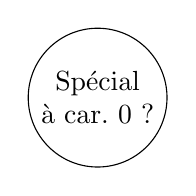
\begin{tikzpicture}\node[draw,circle,inner sep=2pt]{\shortstack{\unsure{Spécial}\\à car.\ 0 ?}};\end{tikzpicture}}
\deleted{définit un op. diff.}
\uline{se factorise de façon canonique en}
\diagram{\begin{tikzcd}[column sep=large]
\underline g \arrow[r,"{c=d^0}"] \arrow[rr,bend right=30,"D"'] & Z^1C_{S/R}(\underline g) \arrow[r,no head,"{\widetilde D}"] & M
\end{tikzcd}}

($\widetilde D$ est loc. induit par un op. diff. sur $\underline g\otimes\Omega^1_{S/R}$ ; \deleted{\unsure{donc les}} \inserted{\unsure{tous les}} $\Delta$, \deleted{\unsure{\Delta\text{ comme}}} \inserted{avec} $\Delta\circ d^0=D$, ont \unsure{même} restriction à $Z^1C_{\unsure{S}/R}(\underline g)$..)

Donc on trouve un composé
\diagram{\begin{tikzcd}[column sep=large]
\underline{\Gamma}(G) \arrow[r,"{g^{-1}dg}"] \arrow[rr,bend right=30,"{\widetilde{\widetilde D}}"'{draw,circle,inner sep=3pt}] & Z^1C_{S/R}(\underline g) \arrow[r,"{\widetilde D}"] & M
\end{tikzcd}}
\margin{220}
